%================================================================
\chapter{The Bayesian Paradigm}\label{chap:bayesian}
%================================================================

\epigraph{A decision was wise, even though it led to disastrous consequences, if the evidence at hand indicated it was the best one to make; and a decision was foolish, even though it led to the happiest possible consequences, if it was unreasonable to expect those consequences.}{Herodotus, around 500 BC}


The aim of statistical inference is to learn about underlying properties of a population from observed data.  In statistical inference, there are, broadly speaking, two paradigms for the analysis of observed data: \textit{frequentist} inference and \textit{Bayesian} inference. These often differ with each other on the fundamental interpretation of probability. In the frequentist view, the probabilities of events are defined as their relative frequencies in a repeatable objective process, and are thus ideally devoid of opinion. The Bayesian view of probability, on the other hand, is based on the degree of belief about the state of the world, and probabilities can be assigned to any statement, even when a random process is not involved. Bayesian inference is the process of revising beliefs about the state of the world in the light of new evidence.   

This chapter introduces the fundamentals of Bayesian inference, with a particular focus on parameter estimation.




%================================================================
\section{Bayesian Inference}\label{sec:bayes_paradigm}
%================================================================

In terms of parameter estimation, the Bayesian approach to inference differ from the frequentist in that unknown parameters $\theta$ are treated as random variables rather than fixed quantities. In the Bayesian paradigm, all available information about an unknown parameter is incorporated in a \textit{prior probability distribution}, expressing our beliefs before some evidence is taken into account. We usually have a prior pdf $\pi(\theta)$, since there will typically be a continuum of possible values of a parameter rather than just a discrete set \cite[p. 758, 776]{STK}. In the case of substantial prior knowledge about a parameter $\theta$, the prior pdf is narrow and concentrated about some central value, whereas a lack of information yield a wider and relatively flat prior pdf as shown in \autoref{fig:prior_illustration}. The prior is often specified by a particular distribution among a set of well-known and tractable distributions, with the purpose of making evaluation of prior probabilities and random generation of $\theta$ values straightforward \cite{ABCprimer}.

\begin{figure}[H]
    \centering
    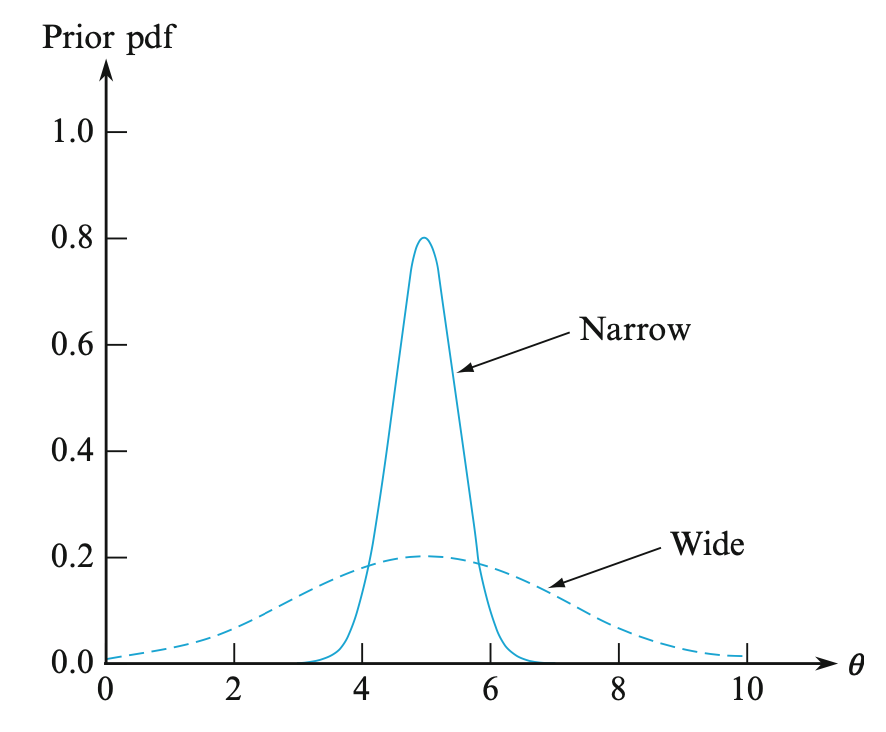
\includegraphics[scale=0.6]{./3_Images/prior_illustration.png}
    \caption{A narrow concentrated prior about some central value and a wider less informative prior.}
    \label{fig:prior_illustration}
    \source{Figure 14.3 in \cite{STK}.}
\end{figure}


Our prior state of knowledge is modified by data $y$, obtained by performing experiments, through the conditional \textit{sampling distribution} $p (y \mid \theta)$, which is called the \textit{likelihood function}. In order to make probability statements about $\theta$ given sample data $y$, a probabilistic model representing the joint probability distribution for $\theta$ and $y$ must be provided \cite[p. 6]{BDA}. The joint pmf or pdf can be written as a product of the prior distribution $\pi(\theta)$ and the likelihood function $p(y \mid \theta)$:

\begin{equation*}
    p(\theta, y) = p(y \mid \theta) \pi(\theta) 
\end{equation*}

At this point, Bayes' theorem is used to produce the \textit{posterior distribution}, which represents our state of knowledge about $\theta$ in the light of $y$ \cite[p. 6]{Sivia}. A common incarnation of Bayes' theorem is

\begin{equation}\label{eq:bayes_theorem}
    \pi \left( \theta \mid y\right) = \frac{p(\theta, y)}{p(y)}  = \frac{p \left(y \mid \theta \right) \pi \left(\theta \right)}{p(y)}
\end{equation}

The quantity $p(y)$ is called the \textit{evidence} and is the distribution of the observed data marginalized over the parameter \cite{ABCprimer}. In the case of continuous $\theta$ the evidence is given by $p(y) = \int p(y \mid \theta) \pi(\theta) \mathrm{d}\theta$, and in the case of discrete set of parameters by $p(y) = \sum_\theta p(y\mid \theta) \pi(\theta)$, where the sum is over all possible values of $\theta$ \cite[p. 7]{BDA}. 

The evidence is the same for all possible $\theta$, as it does not depend on $\theta$, meaning that, with fixed $y$ this factor can be omitted in parameter estimation since it constitutes a normalizing constant and does not enter into determining the relative posterior probabilities of different values of $\theta$ \cite{ABCprimer}. Omitting the evidence yields the unnormalized posterior distribution: 

\begin{equation}\label{eq:bayes_unnorm}
    \pi (\theta \mid y) \propto p(\theta, y) =  p (y \mid \theta) \pi (\theta)
\end{equation}

In this formulation, $p \qty(y \mid \theta)$ is taken as a function of $\theta$ and not $y$.  

The core of Bayesian inference is encapsulated in \autoref{eq:bayes_theorem} and \autoref{eq:bayes_unnorm}. The principal task is to develop the joint probability model $p(\theta, y)$ and perform the computations to summarize the posterior $\pi(\theta \mid y)$.


%================================================================
\section{The Coin-flipping Problem}\label{sec:coin_flipping}
%================================================================

The way in which Bayes’s theorem operates is best seen through examples. 


%================================================================
\section{Toy Problems for Benchmarking}\label{sec:toy_problems}
%================================================================

Develop problems for benchmarking

%================================================================
\subsection{The Coin-flipping Problem}\label{sec:coin_flipping}
%================================================================

Only derive this

%================================================================
\subsection{Gaussian Models}\label{sec:gaussian_models}
%================================================================

normal models important blabla

%================================================================
\subsubsection{With Unknown Mean}
%================================================================

The comprehensive derivation can be found in appendix B. 

Devore, p. 781 

Note that the posterior mean $\mu_0'$ is a weighted average of the prior mean $\mu_0$ and the data mean $\bar{x}$, with weights that are the reciprocals of the prior variance and the variance of $\bar{x}$. It makes sense to define the \textbf{precision} as the reciprocal of the variance because a lower variance implies a more precise measurement and the weights then are the corresponding precisions. Furthermore, the posterior variance is the reciprocal of the sum of the reciprocals of the two variances, but this can be described much more simply by saying that the posterior precision is the sum of the prior precision plus the precision of $\bar{x}$. 

%================================================================
\subsubsection{With Unknown Variance}
%================================================================

The comprehensive derivation can be found in appendix B. 

%================================================================
\subsubsection{With Unknown Mean and Variance}
%================================================================

The comprehensive derivation can be found in appendix B. 


\section{Topics} 

In Bayesian inference, posterior beliefs about parameters are updated according to \textit{Bayes' theorem} upon observing data.  

The mean of this posterior distribution gives a point estimate of $\theta$. 

An interval having a posterior probability $.95$ gives a $95\%$ \textit{credibility} interval, an interval within which an unobserved parameter value falls with a particular probability, the Bayesian analogue of a $95\%$ confidence interval \cite[p. 777]{STK}.

Credible intervals 

HDI 

Energy